\chapter{Estado del Arte}
\label{cap:estadoDelArte}

Una vez planteados los objetivos generales y específicos para este proyecto en la Introducción, este capítulo analiza en mayor profundidad los aspectos clave sobre los que se ha diseñado y construido la solución propuesta. Para ello, primero se amplía el contexto de la escalada explicando su auge en los últimos años se desarrollan los sistemas de dificultad y se definen los desafíos técnicos que conlleva el registro de la actividad. Finalmente, se analiza el panorama tecnológico y se obtienen conclusiones y resultados.

\section{El auge de la escalada en España}

En los últimos años, la escalada ha experimentado un crecimiento sin precedentes a nivel global, principalmente impulsado por su debut como deporte en el calendario olímpico de los Juegos de Tokio 2020. En España, este fenómeno ha sido especialmente notable en parte debido al oro obtenido en estos juegos olímpicos por el escalador Alberto Ginés. El número de licencias de la Federación Española de Deportes de Montaña y Escalada (FEDME) ha crecido de forma exponencial, superando las 290.000 licencias y consolidándose en la actualidad como la cuarta federación deportiva del país \cite{auge_escalada_levante}.

Este auge ha provocado el aumento de rocódromos en los centros urbanos, haciendo de la escalada un deporte mucho más accesible para principiantes al ofrecer un entorno controlado e independiente de las condiciones meteorológicas de la roca. Debido a la popularización del deporte muchos nuevos grupos y perfiles se han introducido a la escalada, lo que resalta la importancia de que las nuevas herramientas se desarrollen con un Diseño Centrado en el Usuario para cubrir las necesidades de estos y aportar un valor real.

\section{Escalas de dificultad y análisis de progresión}

Para poder registrar la actividad deportiva de forma objetiva, la escalada emplea sistemas que categorizan la dificultad de cada ruta. Según los estudios de estandarización, la definición de "difícil" varía enormemente según el nivel del individuo, por lo que las escalas permiten subdividir la exigencia física y técnica en numerosos grados reconocibles por la comunidad \cite{mandelli2019scales}.

Como se introdujo en el capítulo anterior, las escalas más empleadas en España son la Fontainebleau para bloque y la escala francesa para vías. Estas escalas tienen una nomenclatura similar de forma que se estructuran mediante un sistema compuesto por un número, una letra y opcionalmente el símbolo «+». El número (generalmente mayor que 4) define la dificultad base. Esta dificultad se subdivide utilizando las letras «a», «b» y «c» y se emplea el signo positivo para indicar un nivel de dificultad por encima. Como ejemplo una progresión típica sería 6a, 6a+, 6b, 6b+, 6c, 6c+, 7a, y así sucesivamente. Aunque estas dos escalas (francesa y fontainebleau) tengan una notación similar se pueden distinguir de forma que la escala de Fontainebleau suele representarse con letras mayúsculas (por ejemplo, 7B+), mientras que la francesa utiliza minúsculas (por ejemplo, 7b+).

Además de estas escalas a nivel internacional coexisten diversas métricas dependiendo de la modalidad (vía y bloque) y la región geográfica. Destacan el Sistema Yosemite Decimal (YDS) para vías o la escala V (\textit{V-Scale}) para bloque, muy populares en Norteamérica y otras regiones.

Esta variedad de sistemas genera una importante barrera de entrada para los escaladores noveles, ya que la conversión entre escalas no es directa ni matemáticamente exacta. Cada métrica nació en diferentes contextos por lo que como resultado se tienen equivalencias aproximadas y a menudo subjetivas. En consecuencia, los escaladores se encuentran con dificultades para interpretar la dificultad real de rutas al enfrentarse a nomenclaturas extranjeras. Esta falta de estandarización obliga a depender de tablas de conversión externas como la que se observa en la imagen \ref{fig:conversion_dificultades} reduciendo la fluidez del registro de la progresión.

\begin{figure}[h]
    \centering
    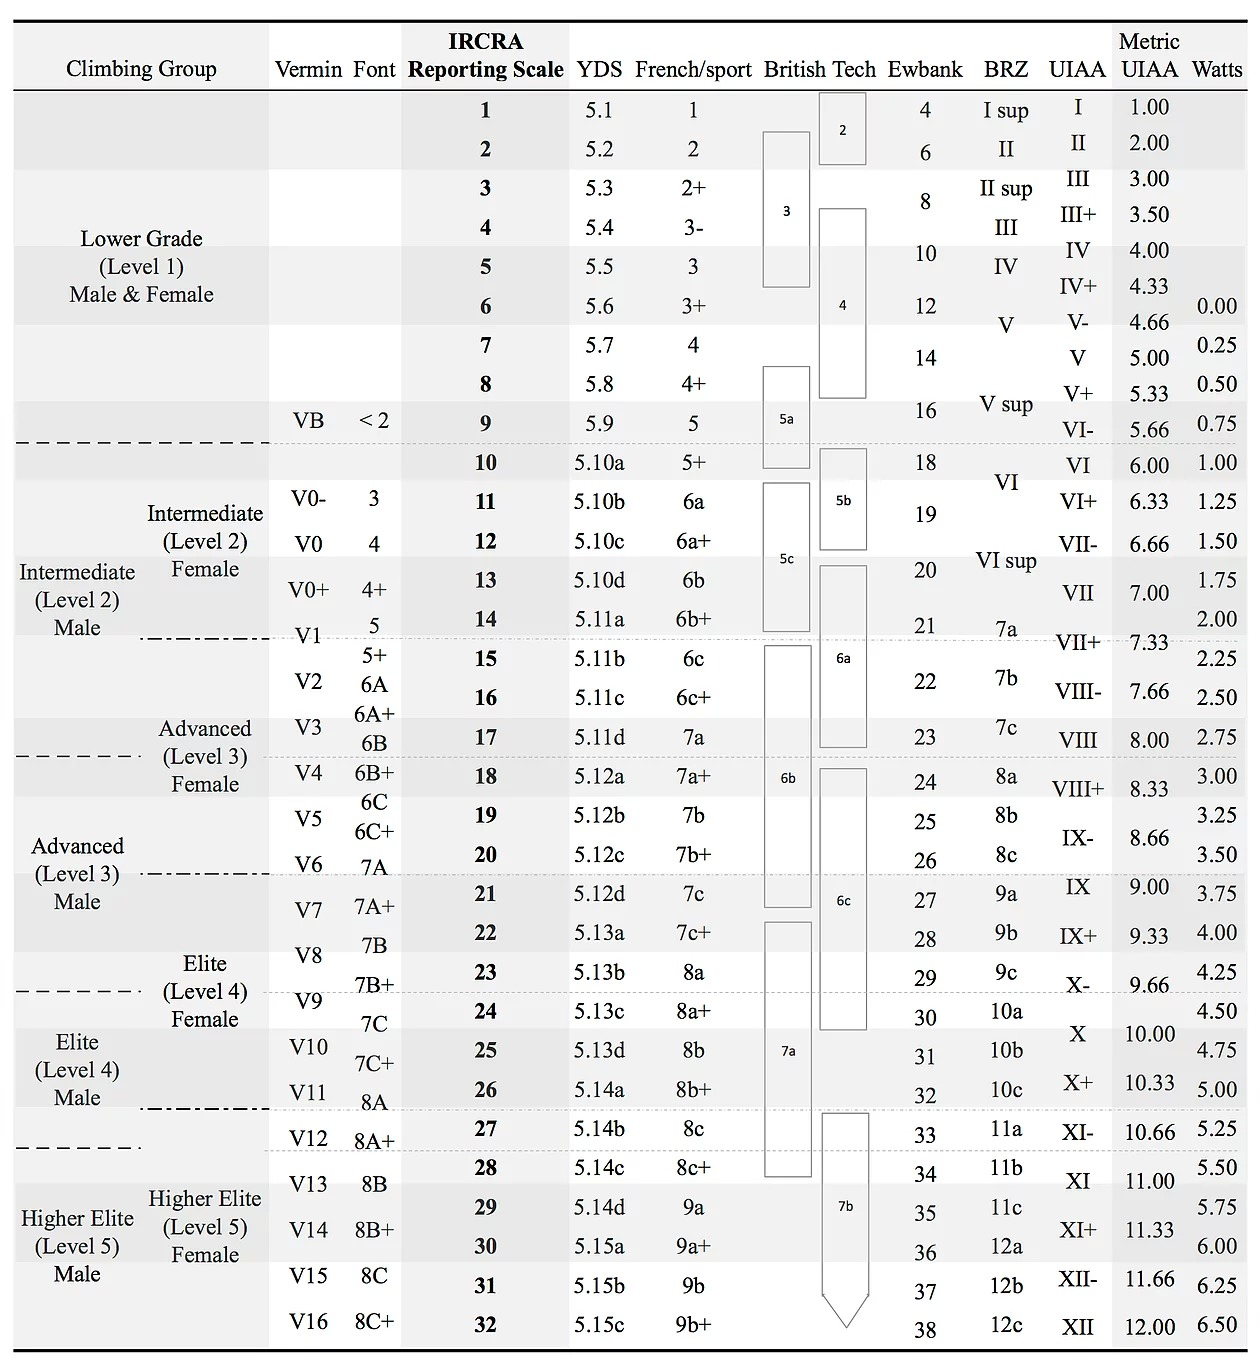
\includegraphics[width=0.8\textwidth]{./Imagenes/Fuentes/conversion_dificultades.jpg} 
    \caption{Tabla de conversión de dificultades.}
    \label{fig:conversion_dificultades}
\end{figure}

\subsection{El progreso en la escalada: Análisis de datos masivos}

El progreso en la escalada es notablemente lento, lo que justifica la necesidad de integrar mecánicas de gamificación para mantener la motivación en los escaladores. En un análisis estadístico sobre 4 millones de ascensiones registradas por \cite{masullo_climbing}, se extraen conclusiones sobre la evolución de los escaladores. Los datos muestran que el 90\% de los usuarios registra a lo largo de su historial entre 3 y 306 ascensiones, situándose la media en unas 110 rutas. Además, como se visualiza en la gráfica \ref{fig:grafica_dificultades_años}, el estudio determina el tiempo promedio que tarda un escalador en superar barreras de dificultad como alcanzar el grado 7a requiere una media de 4,5 años de práctica, llegar al 7b toma unos 6 años y escalar un 8a conlleva entre 8 y 9 años de dedicación.

\begin{figure}[h]
    \centering
    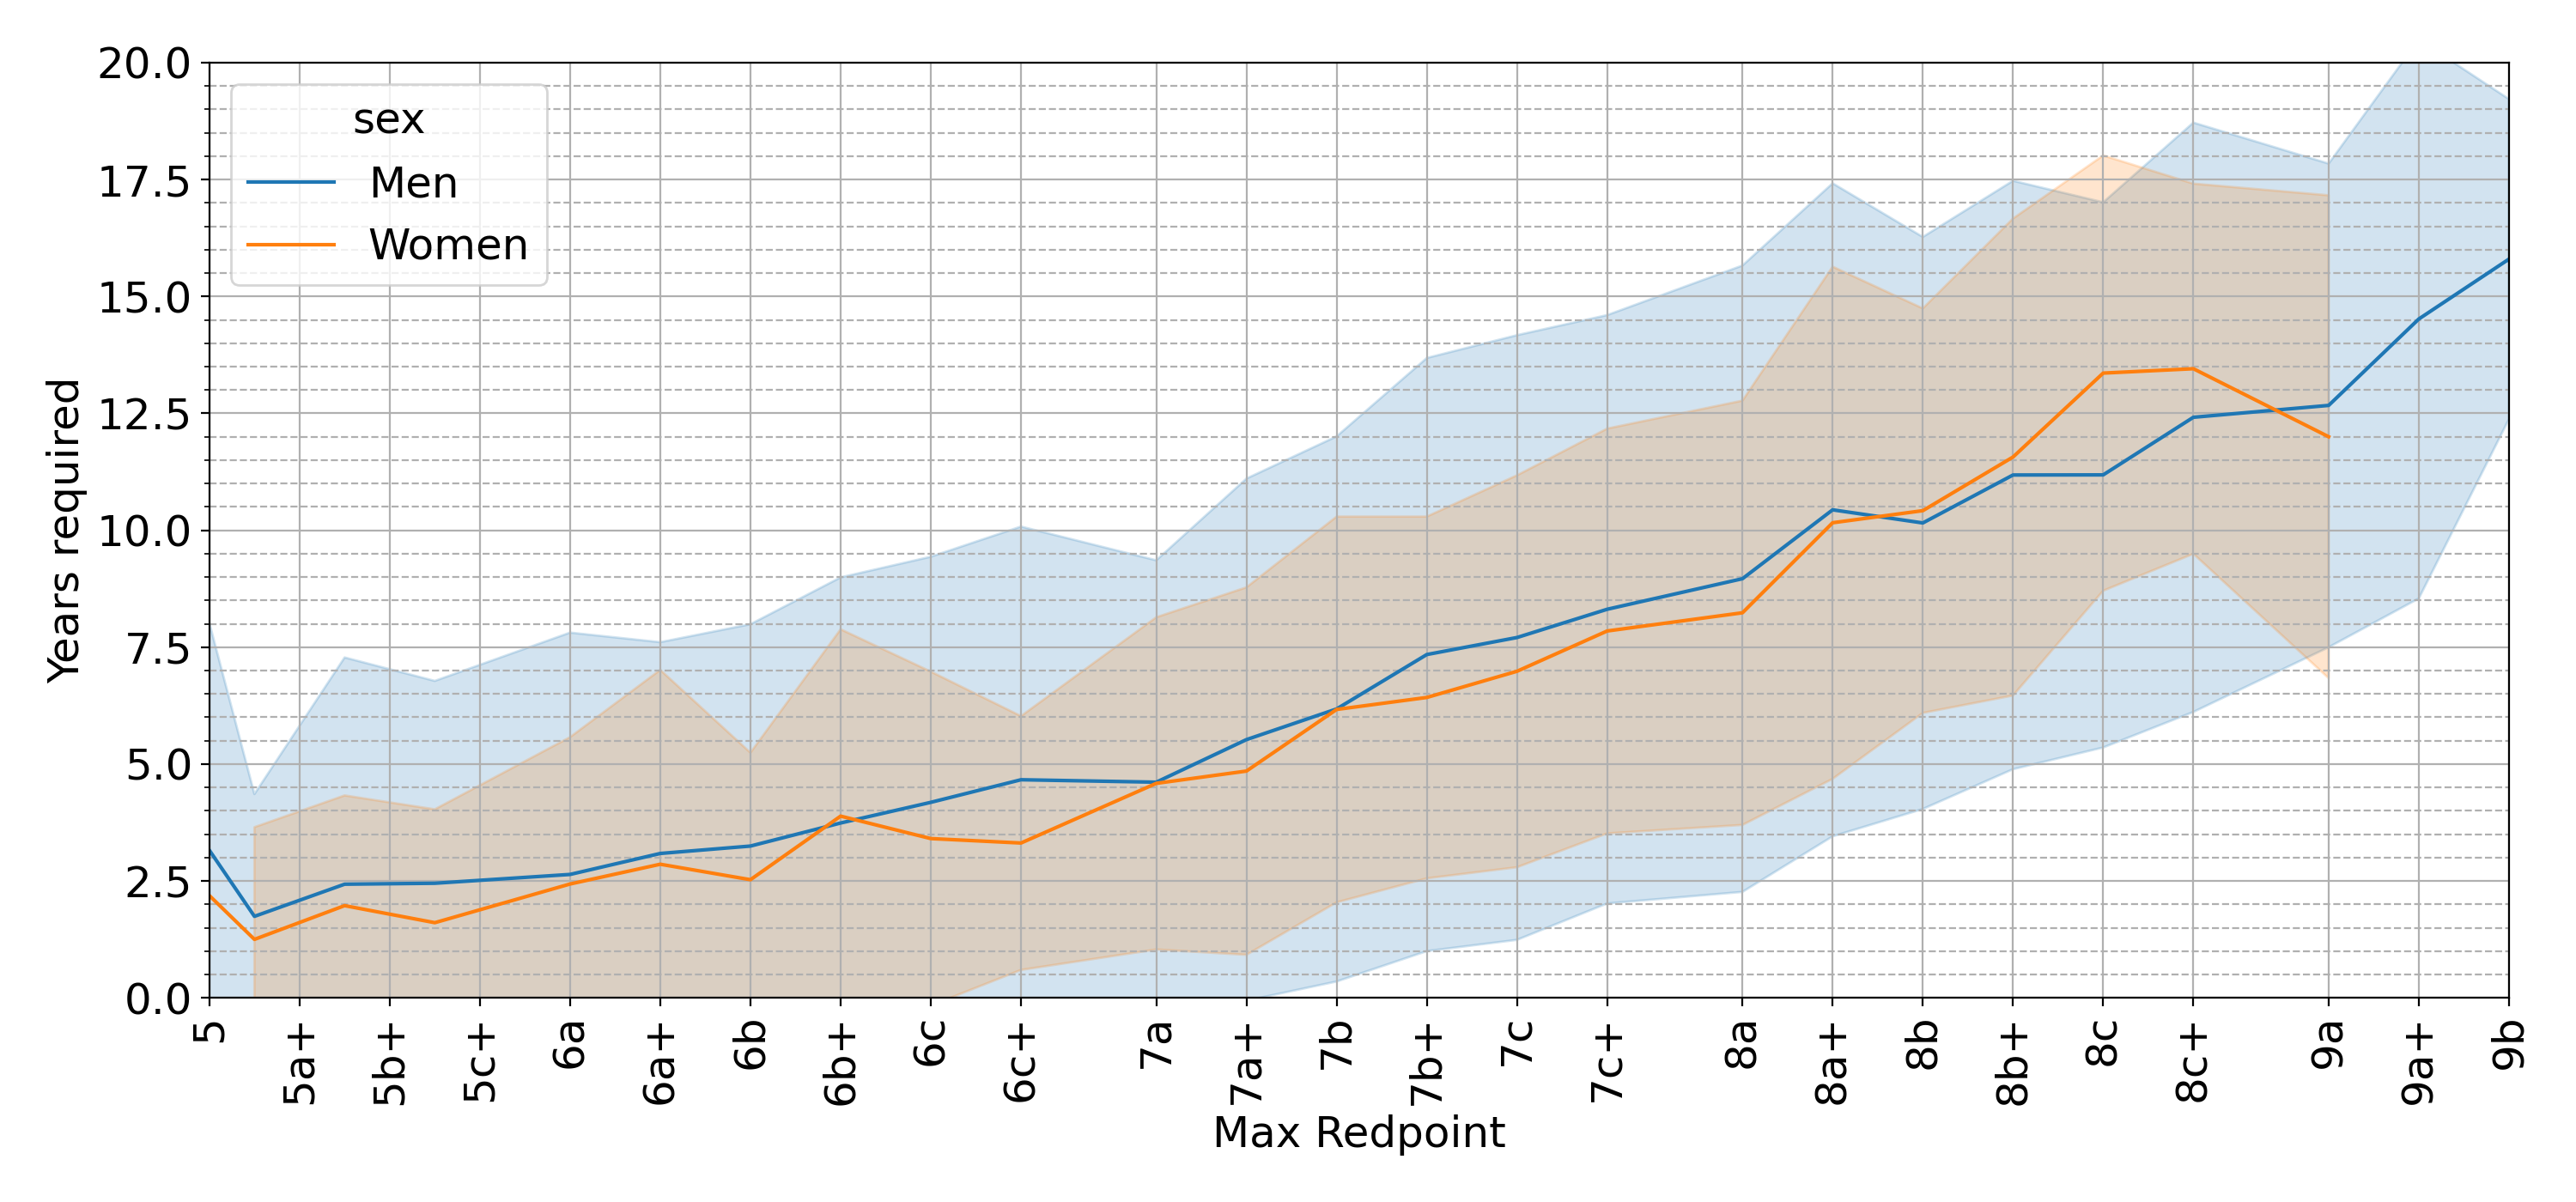
\includegraphics[width=0.8\textwidth]{./Imagenes/Fuentes/dificultad_por_año.png} 
    \caption{Media de dificultades por años escalados.}
    \label{fig:grafica_dificultades_años}
\end{figure}

El análisis también destaca el salto de dificultad que supone subir una ruta ensayada (completada tras varios intentos) frente a conseguirla al \textit{flash} (al primer intento y sin caídas). Por ejemplo, para consolidar un nivel de 7a ensayado, las estadísticas indican que el escalador debe ser capaz de escalar consistentemente grados 6a+/6b al \textit{flash}.

Esta extensa ventana de progreso genera largas fases de estancamiento donde el registro pierde sentido si no cuenta con incentivos a corto y medio plazo, lo que da pie a las soluciones tecnológicas y de gamificación.

\section{Desafíos técnicos en el registro de la actividad}

Mientras que en otros deportes el registro de datos es automático gracias al uso de dispositivos de hardware estandarizados (como el seguimiento de rutas por GPS en ciclismo o el uso de pulsómetros en \textit{running}), en la escalada la situación es significativamente distinta. La inmensa variedad de modalidades, de secuencias de movimientos y de escalas de medición exige que la recolección de los datos dependa de un esfuerzo manual por parte del usuario, lo que suele derivar en la pereza y el abandono del seguimiento.

Para comprender el análisis de las aplicaciones de mercado, es necesario profundizar en esta complejidad técnica. El registro digital debe ser capaz de diferenciar métricas clave como el tipo del ascenso (un ascenso al \textit{flash} aporta mucho más valor que uno ensayado tras múltiples intentos), a la vez que la plataforma debe gestionar de manera fluida la constante rotación periódica de rutas temporales que diseñan los \textit{route setters} del rocódromo.

\section{Análisis de aplicaciones de escalada}

Tras realizar un análisis no exhaustivo de las aplicaciones y soluciones existentes, se han identificado tres tipos de soluciones principales, agrupadas según su propósito funcional:
\begin{itemize}
\item \textbf{Aplicaciones integradas con el rocódromo}
\item \textbf{Aplicaciones centradas en la comunidad}
\item \textbf{Aplicaciones con hardware específico} 
\end{itemize}

En los siguientes subapartados se describen las características técnicas de cada categoría y se realiza un análisis crítico de las fortalezas y debilidades de las aplicaciones identificadas.

\subsection{Aplicaciones integradas con el rocódromo}

Estas aplicaciones mantienen una vinculación directa con las instalaciones deportivas, funcionando como una extensión digital para el registro de la actividad diaria.

\paragraph{TopLogger}
TopLogger\footnote{TopLogger disponible en: \url{https://toplogger.nu/es}} permite el registro del estado de las rutas (completada, flash, proyecto) de los rocódromos asociados, facilitando su identificación por ubicación, color y grado de dificultad. Para la navegación, emplea un mapa cenital interactivo que permite al usuario desplazarse por los diferentes sectores del muro como se aprecia en la imagen \ref{fig:toplogger_mapa}y al ampliar se muestran las rutas de cada zona como se aprecia en la imagen \ref{fig:toplogger_rutas}.

\begin{figure}[h]
    \centering
    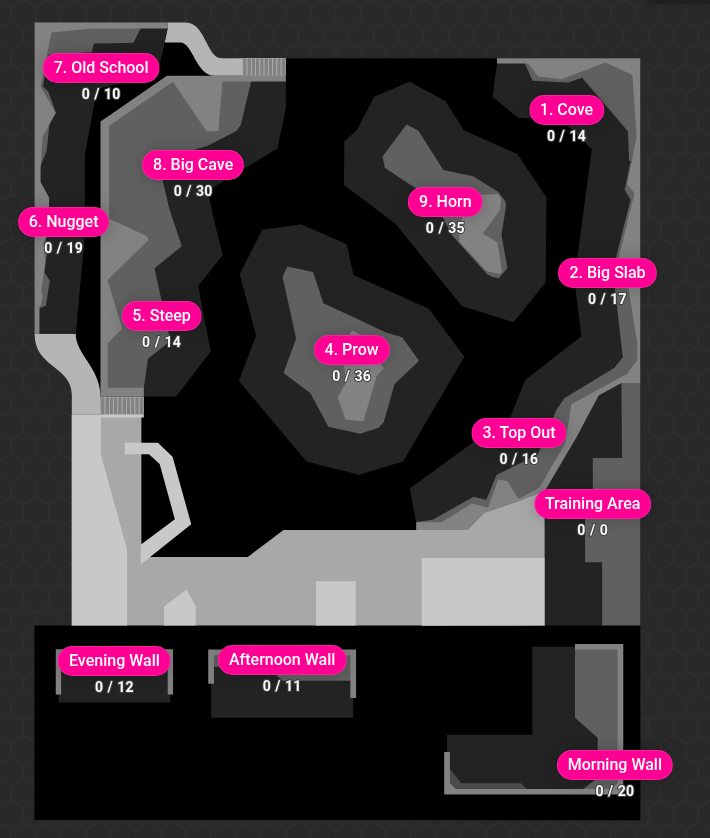
\includegraphics[width=0.6\textwidth]{./Imagenes/Fuentes/toplogger_mapa.png} 
    \caption{Sectores en el mapa cenital de TopLogger.}
    \label{fig:toplogger_mapa}
\end{figure}

\begin{figure}[h]
    \centering
    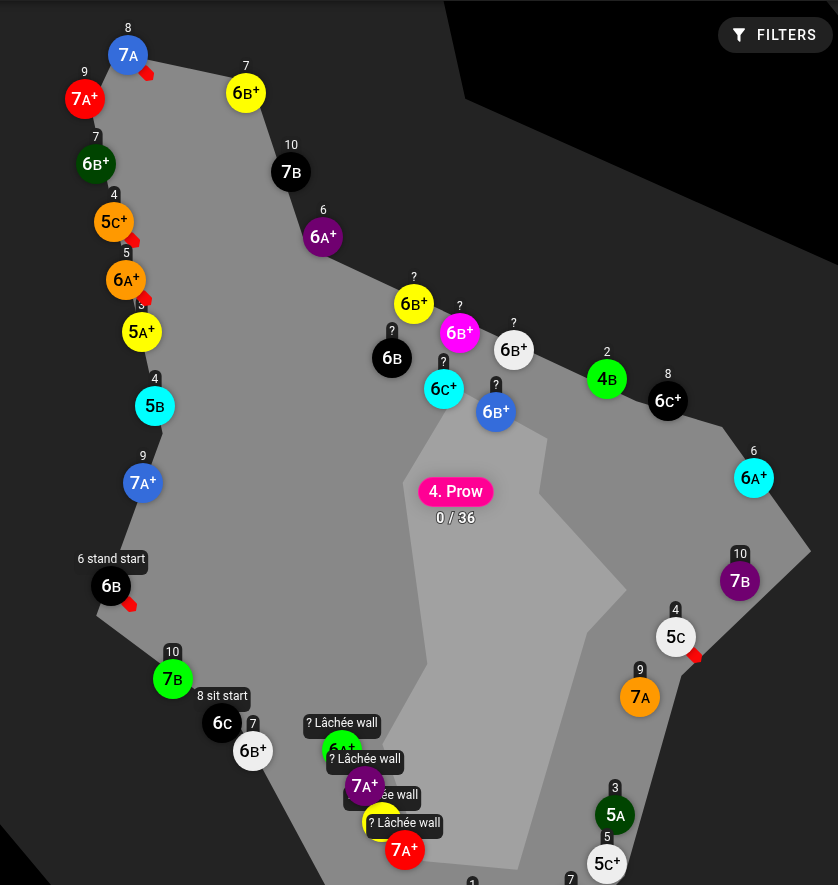
\includegraphics[width=0.6\textwidth]{./Imagenes/Fuentes/toplogger_rutas.png} 
    \caption{Rutas en el mapa cenital de TopLogger.}
    \label{fig:toplogger_rutas}
\end{figure}

La aplicación ofrece estadísticas detalladas sobre las sesiones de escalada y un sistema de gamificación basado en niveles y clasificaciones por centro. No obstante, presenta una notable sobrecarga de información en su interfaz, lo que compromete la usabilidad para perfiles con menor competencia tecnológica. Además, su sistema de ránkings es vulnerable a registros falsos y su implantación en España es actualmente limitada.

\paragraph{WeClimb}
WeClimb\footnote{WeClimb disponible en: \url{https://weclimb.fr/}} ofrece funcionalidades de registro similares a TopLogger, pero se diferencia por su sistema de identificación de rutas está basado en tarjetas visuales con fotografías reales de las rutas. Esta aproximación facilita el reconocimiento del bloque o la vía directamente frente al muro.

\begin{figure}[h]
    \centering
    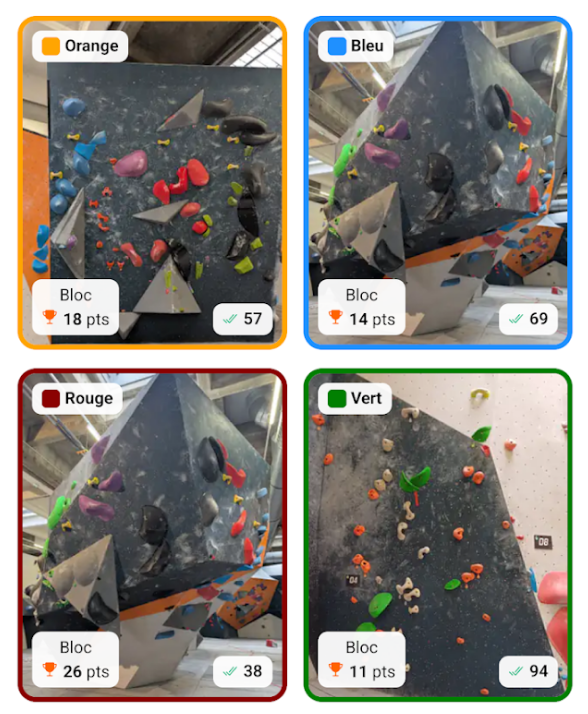
\includegraphics[width=0.6\textwidth]{./Imagenes/Fuentes/weclimb_tarjetas.png} 
    \caption{Sistema de tarjetas de WeClimb.}
    \label{fig:weclimb_tarjetas}
\end{figure}

Incluye herramientas para resaltar las presas utilizables en cada imagen, permitiendo la creación de retos personalizados. Sin embargo, su despliegue está focalizado en el mercado francés y carece de una capa de gamificación profunda. Asimismo, la navegación por tarjetas puede resultar ineficiente en muros con una densidad de rutas muy elevada.

\subsection{Aplicaciones centradas en la comunidad}

Aplicaciones que priorizan la interacción social y el intercambio de experiencias sobre el registro de cada ascenso.

\paragraph{KAYA}
KAYA\footnote{KAYA disponible en: \url{https://kayaclimb.com/}} se trata de una red social orientada a la escalada, donde los usuarios comparten sus ascensos mediante publicaciones y vídeos cortos en formato vertical, conocidos como \textit{betas}, con una estructura similar a aplicaciones como \textit{Instagram} como se aprecia en la imagen \ref{fig:kaya_profile}. Implementa un sistema de gamificación de insignias (\textit{Badges}) en base al número de rutas completadas y su dificultad como se observa en la imagen \ref{fig:kaya_badges}. Su principal limitación es que está orientada a ascensos puntuales generalmente en roca natural, careciendo de una integración fluida con rocódromos.

\begin{figure}[h]
    \centering
    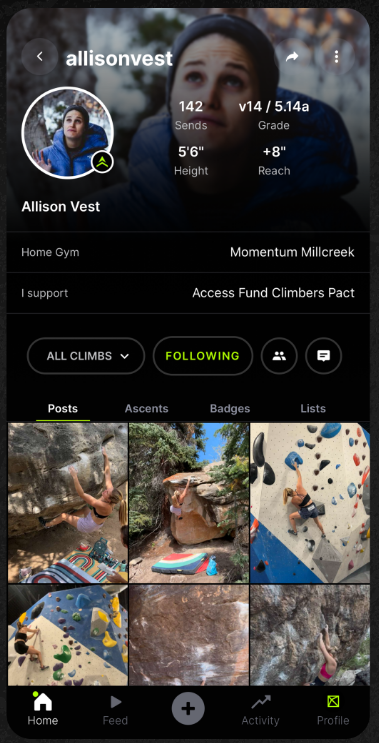
\includegraphics[width=0.4\textwidth]{./Imagenes/Fuentes/kaya_profile.png} 
    \caption{Perfil de la escaladora Allison Vest en Kaya.}
    \label{fig:kaya_profile}
\end{figure}

\begin{figure}[h]
    \centering
    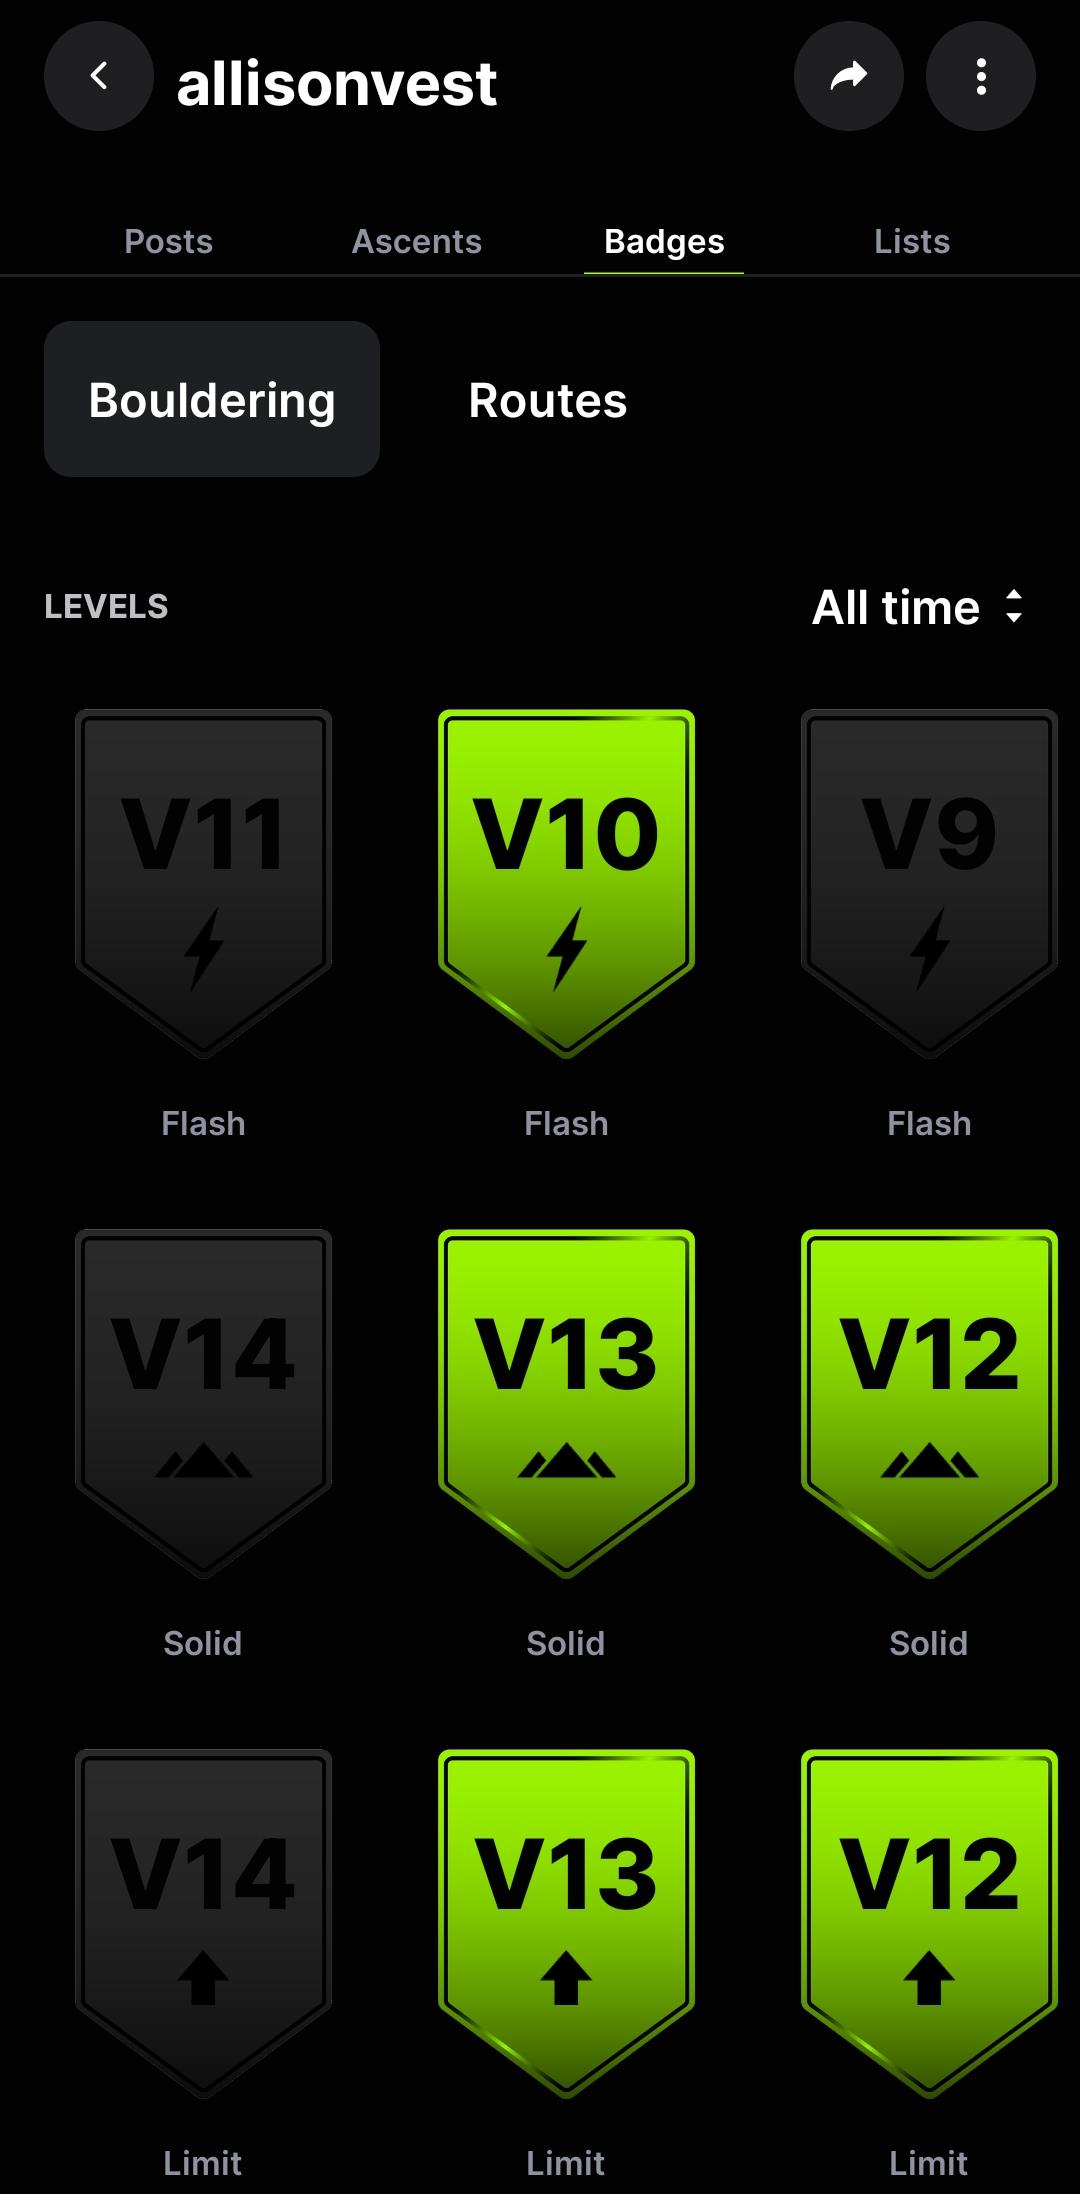
\includegraphics[width=0.4\textwidth]{./Imagenes/Fuentes/kaya_badges.jpeg} 
    \caption{Logros del escalador en KAYA.}
    \label{fig:kaya_badges}
\end{figure}

\subsection{Aplicaciones con hardware específico}

\paragraph{Kilter Board}
Kilter Board\footnote{Kilter Board disponible en: \url{https://kilterboard.io/}} es una solución híbrida que combina un muro físico estandarizado con un sistema de iluminación LED controlado por una aplicación móvil que al seleccionar una ruta en la app, las presas correspondientes se iluminan en el muro como se observa en la imagen \ref{fig:kilterboard}.

\begin{figure}[h]
    \centering
    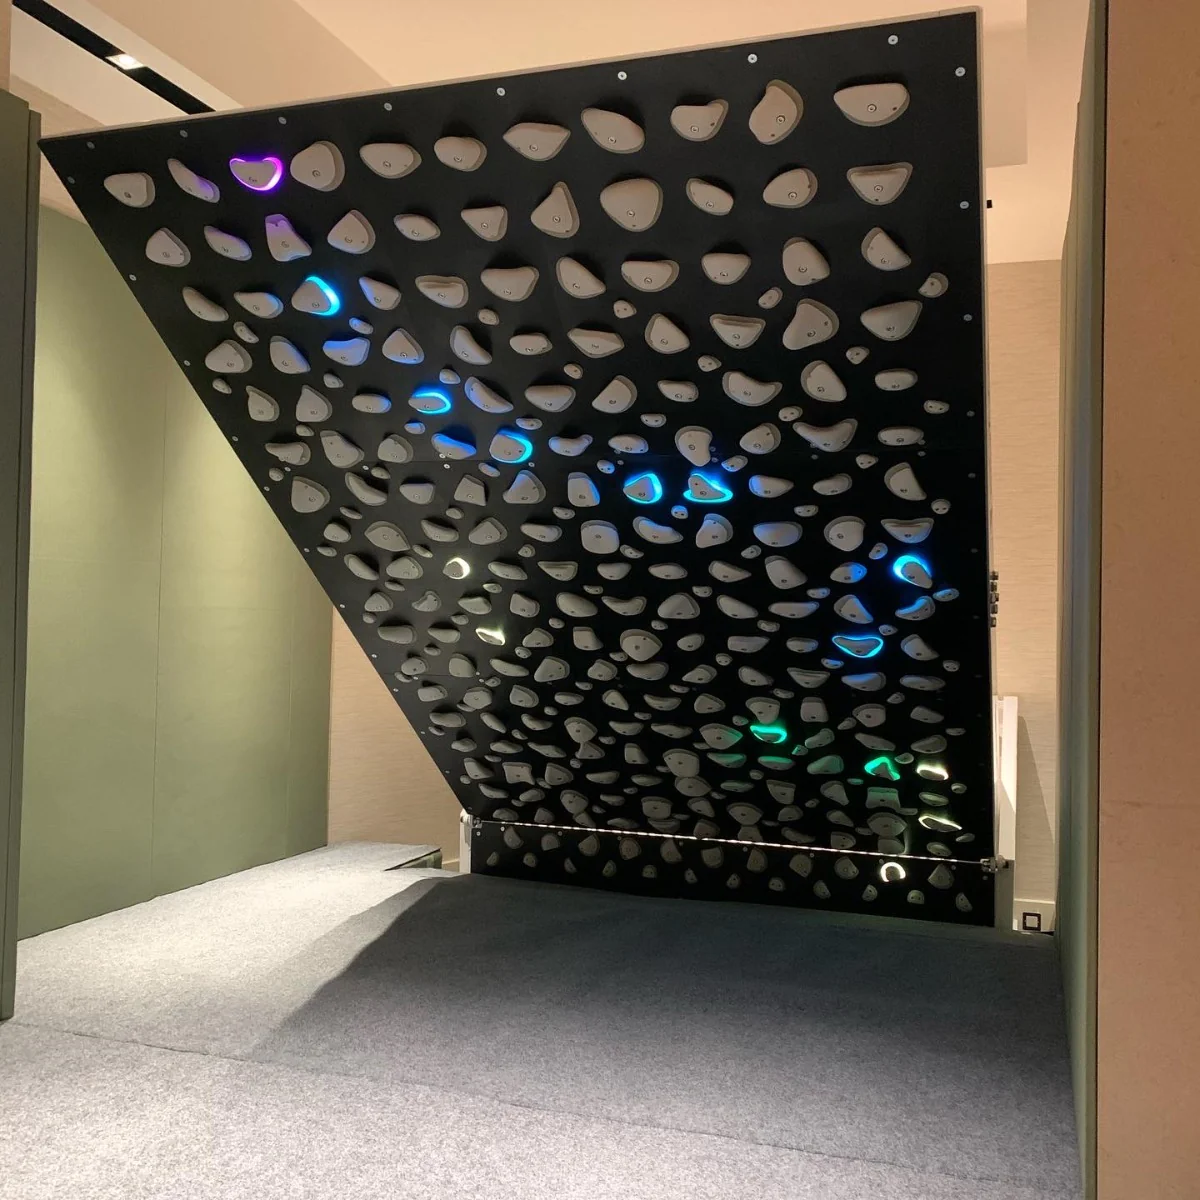
\includegraphics[width=0.7\textwidth]{./Imagenes/Fuentes/muro_kilter.png} 
    \caption{Sistema Kilter Board.}
    \label{fig:kilterboard}
\end{figure}

Cuenta con un sistema de \textit{ranking} global y una extensa base de datos validada por la comunidad, permitiendo la comparación de rendimiento a nivel mundial. A diferencia de otras herramientas orientadas únicamente al alto rendimiento (como MoonBoard), destaca por su diseño ergonómico y su accesibilidad para escaladores principiantes, en gran parte gracias a la posibilidad de ajustar la inclinación del muro. Su limitación es que su uso se limita exclusivamente a su hardware específico realizando un registro parcial.

\section{Análisis de aplicaciones de otros deportes}

Para identificar mecánicas de gamificación transferibles, se han examinado aplicaciones de éxito en otros sectores deportivos.

\subsection{Competiciones y ranking por segmentos (Strava)}
Strava \footnote{Strava disponible en: \url{https://www.strava.com/}} ha logrado una alta fidelización de usuarios mediante el concepto de "segmentos"(tramos específicos de una ruta donde los usuarios comparan tiempos registrados vía GPS). Sus títulos (KOM/QOM) son un sistema de badges para transformar el entrenamiento en una competición virtual. Este modelo se puede extrapolar a la escalada tratando cada vía o bloque como un segmento donde medir el número de intentos o el estilo de ascenso. A pesar de que existe una modalidad de escalada basada en el tiempo en completarla, el registro basado en el tiempo es contraproducente en esta disciplina, ya que puede comprometer la técnica y la seguridad del escalador en favor de la velocidad.

\subsection{Coleccionismo de logros (Pokémon Go)}
Pokémon Go\footnote{Pokémon Go disponible en: \url{https://pokemongo.com/es}} destaca por la implementación del sistema PBL (Points, Badges and Leaderboards) vinculado al coleccionismo y al desplazamiento físico. Esta mecánica de completar colecciones es aplicable a la escalada mediante un sistema de recompensas basado en el esfuerzo realizado incentivando la constancia y el descubrimiento de nuevas rutas. La principal desventaja de este enfoque es el riesgo de generar una dependencia negativa en el usuario, provocando que el objetivo principal deje de ser la actividad deportiva para centrarse únicamente en la obtención de esta recompensa virtual.

\section{Conclusiones del Estado del Arte e identificación de la oportunidad}
 
Para finalizar en este capítulo se presentan las conclusiones obtenidas tras el análisis comparativo entre las aplicaciones, permitiendo identificar la necesidad del mercado y la propuesta de valor de nuestra aplicación.

\subsection{Síntesis de la problemática actual}

Tras analizar el contexto y las soluciones existentes, se observa que las soluciones actuales para la escalada presentan los siguientes aspectos críticos:

\begin{itemize}
\item \textbf{Experiencia de Usuario (UX) deficiente:} Aplicaciones como TopLogger o WeClimb ofrecen una gran densidad de datos, pero a costa de interfaces saturadas que dificultan el uso y registro de rutas en la aplicación. La barrera tecnológica aleja al escalador casual que solo busca un registro sencillo de su progresión.
\item \textbf{Gamificación superficial:} La mayoría de las herramientas se limitan a clasificaciones numéricas (leaderboards) fácilmente manipulables, lo que genera desmotivación.
\item \textbf{Dependencia de hardware o geografía:} Existen buenas soluciones como Kilter Board, pero están limitadas a sus muros de escalada específicos dando como resultado un registro parcial de las sesiones de escalada.
\item \textbf{Escalas de dificultad no normalizadas:} La gran variedad de escalas diferentes crea una barrera de accesibilidad para determinar la dificultad real de una ruta, causando que las aplicaciones solo acepten un tipo de escala y perjudicando a una fracción de los usuarios.
\end{itemize}

\subsection{Limitaciones de las soluciones existentes y oportunidades de mejora}

El análisis de aplicaciones como \textbf{Strava} y \textbf{Pokémon Go} revela que existe un gran potencial en la adaptación de mecánicas de gamificación de otros sectores a la escalada. La oportunidad reside en desarrollar una solución que combine los siguientes factores:

\begin{enumerate}
\item \textbf{Registro visual y ágil:} Adoptar un sistema híbrido de mapas cenitales dinámicos como los de TopLogger y sistema de tarjetas para minimizar el tiempo de interacción de escalador para reconocer y acceder a la ruta con el móvil durante la sesión como los de WeClimb.
\item \textbf{Gamificación basada en PBL:} Realizar una implementación correcta del sistema PBL basado en el modelo RAMP de forma que las estadísticas funcionen como los \textit{Points} para mantener la motivación y constancia de los usuarios, además de la implementación de Leaderboards entre grupos de amigos eliminando el factor de los abusos de los sistemas de posicionamiento.
\item \textbf{Enfoque social y comunitario:} Fomentar la interacción mediante personalización del perfil y la comparación de estadísticas personales, creando un sentimiento de pertenencia a la comunidad del rocódromo local (\textit{Relatedness} del modelo RAMP).
\item \textbf{Sistemas de dificultades personalizados:} Crear un sistema que permita a cada rocódromo tener asignado para bloques y vías una escala de dificultad diferente entre sistemas estandarizados (como escala francesa, Fontainebleau, V-Scale entre otros) o personalizados, reduciendo así la fricción que genera que un centro no pueda usar sus propias escalas.
\item \textbf{Diseño Centrado en el Usuario:} Desarrollar una herramienta basada en las necesidades reales de los usuarios a través de pruebas e iteraciones continuas. El objetivo principal es mitigar las frustraciones comunes de los escaladores principiantes, un segmento en auge debido a la reciente popularización del deporte.
\end{enumerate}

En conclusión, este proyecto se sitúa en un punto medio entre las herramientas de entrenamiento y las redes sociales de deportes. De esta manera se propone una alternativa para los entrenamientos que registra datos de las sesiones de escalada y motiva al escalador mediante una experiencia gamificada y social.